% Created 2025-01-28 Tue 13:14
% Intended LaTeX compiler: pdflatex
\documentclass[11pt]{article}
\usepackage[utf8]{inputenc}
\usepackage[T1]{fontenc}
\usepackage{graphicx}
\usepackage{longtable}
\usepackage{wrapfig}
\usepackage{rotating}
\usepackage[normalem]{ulem}
\usepackage{amsmath}
\usepackage{amssymb}
\usepackage{capt-of}
\usepackage{hyperref}
\usepackage[danish, ]{babel}
\usepackage[margin=2.5cm]{geometry}
\usepackage{lmodern}
\hypersetup{colorlinks, linkcolor=blue, urlcolor=blue}
\author{Alexander Knudsen, Andreas Jensen og Jeppe Bøgeskov}
\date{\today}
\title{Teknologiprojekt -- Fremtidens levevis}
\hypersetup{
 pdfauthor={Alexander Knudsen, Andreas Jensen og Jeppe Bøgeskov},
 pdftitle={Teknologiprojekt -- Fremtidens levevis},
 pdfkeywords={},
 pdfsubject={},
 pdfcreator={Emacs 29.4 (Org mode 9.7.11)}, 
 pdflang={Dk}}
\begin{document}

\newgeometry{top=2.0cm, bottom=2.0cm}
\begin{titlepage}
    \centering

    \vspace*{1cm}

    % Title and subtitle are enclosed between two rules.
    \rule{\textwidth}{1pt}

    % Title
    \vspace{.7\baselineskip}
    {\huge \textbf{Projekt 1 - Krisen kradser}}

    % Subtitle
    \vspace*{.5cm}
    {\LARGE Efterårssemester 2024}

    \rule{\textwidth}{1pt}

    \vspace{1cm}

    % Set this size for the remaining titlepage.
    \large

    % Authors side by side, using two minipages as a trick.

    \begin{table}[h]
        \centering
        \begin{tabular}{cc}
            \begin{minipage}{.5\textwidth}
                \centering
                Jeppe Bøgeskov Bech \\
                {\normalsize \url{jepp9920@zbc.dk}}
            \end{minipage}
            &
            \begin{minipage}{.5\textwidth}
                \centering
                Alexander Schade Knudsen \\
                {\normalsize \url{alex245h@zbc.dk}}
            \end{minipage}
        \end{tabular}

        \vspace{1cm} % Adds vertical space between the rows

        \begin{minipage}{.5\textwidth}
            \centering
            Andreas Jensen \\
            {\normalsize \url{andr328q@zbc.dk}}
        \end{minipage}
    \end{table}








    % More authors can be inserted here with additional minipages.

    \vspace{1cm}

    % Report logo.
    \fbox{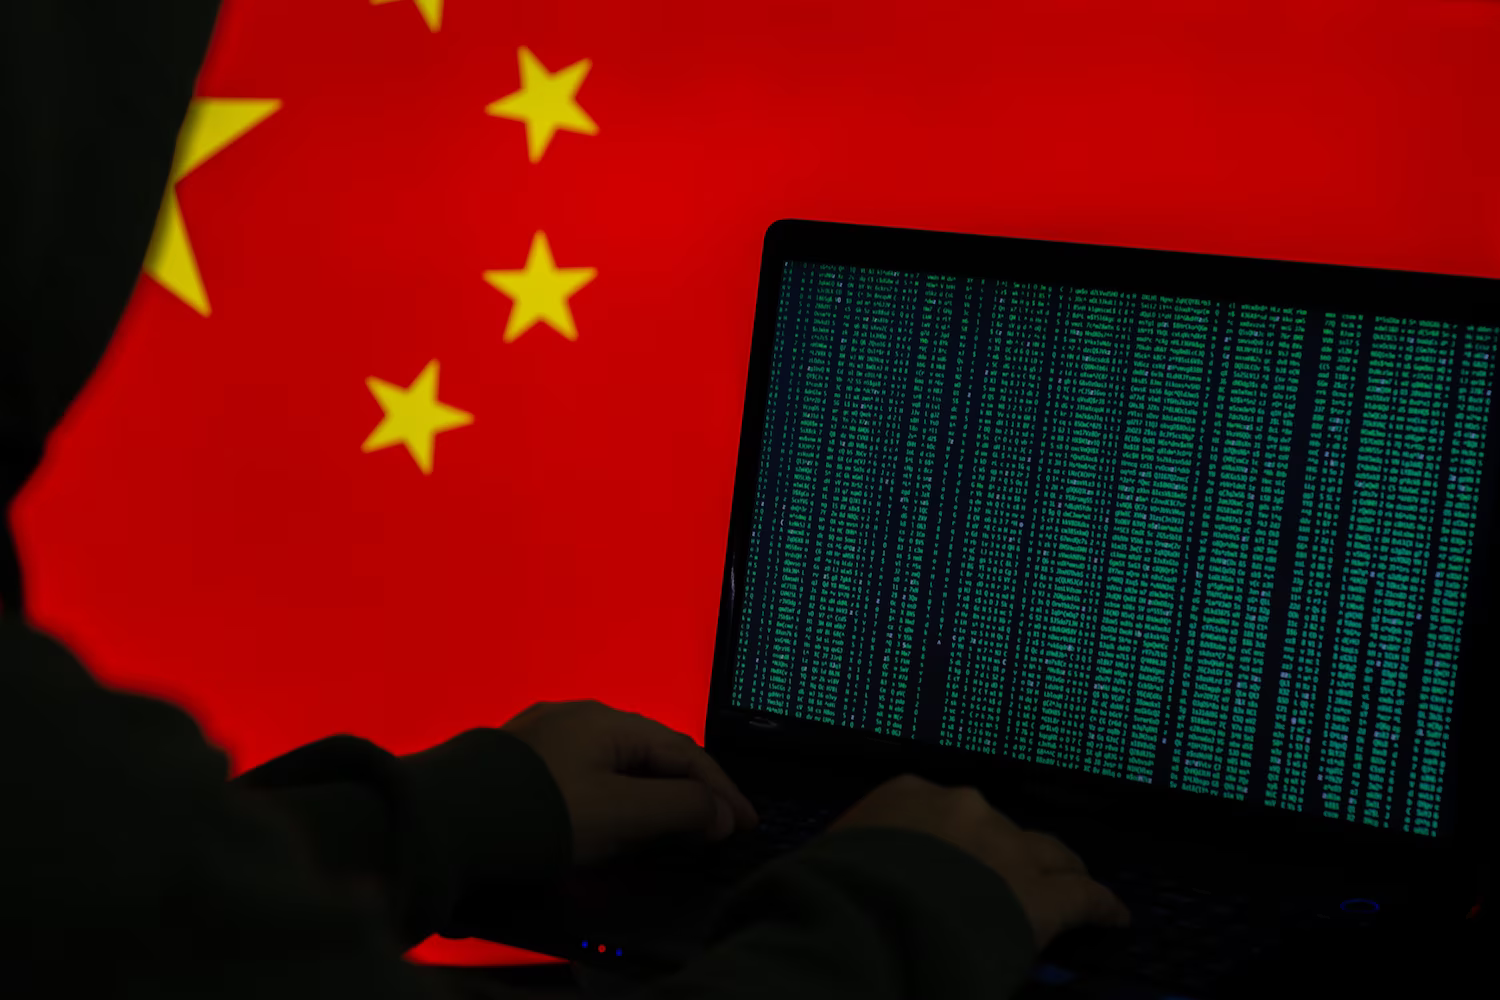
\includegraphics[width=.7\textwidth]{./assets/forsidebillede.png}}

    \vfill

    % University and date information at the bottom of the titlepage.
    2. x \\
    ZBC Handels- og Teknisk gymnasium Slagelse \\
    Akademisk år 2024-2025 \\
    \today
\end{titlepage}


\restoregeometry
\tableofcontents
\newpage
\section{Abstract}
\label{sec:orgb9c23e5}
\section{Forord}
\label{sec:orgc2214df}
\section{Indledning}
\label{sec:org371958f}
\subsection{Projektstyring}
\label{sec:orgff87971}
\subsubsection{Gantt-diagram}
\label{sec:orgdc0c31b}
\subsubsection{Oplæg}
\label{sec:orgacd79b4}
Heri projektet arbejdes der med casen, der omhandler 'bolig'.
\subsection{Problemidentifikation}
\label{sec:orgbbc5899}
\subsubsection{Samfundsmæssige problemstilling}
\label{sec:org23b9d5b}
Den samfundsmæssige problemstilling som heri projektet arbejdes med, er det faktum, at Smart Hjem-løsninger i udstrakt grad suppleres af firmaer med oprindelse i Kina (TODO indsæt kilde). Dette er problematisk, da løsningerne kræver meget data for at fungere, og da de ligge i Kina, kan det kinesisk kommunistiske parti kræve, at disse data indhentes (TODO indsæt kilde).

Udover at det kan være et problem for den individuelle bruger, at vedkommendes data indsamles og anvendes til formål, vedkommenede ikke bryder sig om, så er det også et nationalt sikkerhedsproblem, da disse data kan anvendes til at danne forbrugsmønstre over gruppen af mennesker, hvis data indsamles.
\section{Problemanalyse}
\label{sec:org6aef79d}
\subsection{Interessentanalyse}
\label{sec:orgec7817c}
\subsubsection{Ekstern interessenter}
\label{sec:orge1f4b78}
\begin{itemize}
\item NGO'er
\end{itemize}
\subsubsection{Gidsel}
\label{sec:org7adb390}
\begin{itemize}
\item Konsumenter
\end{itemize}
\subsubsection{Grå eminence}
\label{sec:org8716a33}
\begin{itemize}
\item Konkurrenter
\end{itemize}
\subsubsection{Ressourceperson}
\label{sec:org34ba23e}
\begin{itemize}
\item Staten
\end{itemize}
\subsection{HV-modellen}
\label{sec:orga2f59cc}
\subsubsection{Hvad}
\label{sec:org50be78a}
\begin{enumerate}
\item Et konkurrencealternativ
\end{enumerate}
\subsubsection{Hvorfor}
\label{sec:org8c367e1}
\begin{enumerate}
\item For at få markedsandel på vestlige hænder
\end{enumerate}
\subsubsection{Hvem}
\label{sec:orgdc878a7}
\begin{enumerate}
\item Et privat firma.
\item Kinesiske firmaer påvirkes, her negativt.
\end{enumerate}
\subsubsection{Hvor}
\label{sec:orgfd954fc}
\begin{enumerate}
\item Resten af vestlige lande.
\end{enumerate}
\subsubsection{Hvordan}
\label{sec:orgb429efe}
\begin{enumerate}
\item Decentralt IoT-system
\end{enumerate}
\section{Produktprincip}
\label{sec:orgfbbd55a}
\section{Produktudformning}
\label{sec:org9684031}
\subsection{Software}
\label{sec:org7b64fe2}
\subsection{Hardware}
\label{sec:orgec3b2d2}
\section{Produktionsforberedelse}
\label{sec:org3d99a52}
\subsection{Masseproduktion}
\label{sec:orgc5964ea}
\section{{\bfseries\sffamily TODO} Realisering}
\label{sec:org7d42a1d}
\section{{\bfseries\sffamily TODO} Evaluering}
\label{sec:org6ac19ad}
\section{{\bfseries\sffamily TODO} Miljøvurdering}
\label{sec:org0117987}
\subsection{Hardwarepåvirkning}
\label{sec:org46efe07}
\subsection{Softwarepåvirkning (serverpåvirkning)}
\label{sec:orgf0c9e32}
\section{Konklusion}
\label{sec:org8d5fd2b}
\end{document}
